\documentclass[10pt]{article}
\pdfminorversion=7
\usepackage{icassp2027_paperkit}
\usepackage{amsmath,amssymb,booktabs,graphicx,microtype,url}
\usepackage[T1]{fontenc}
\usepackage{textcomp,balance,capt-of}
\usepackage[hidelinks]{hyperref}
\urlstyle{same}
\hypersetup{pdftitle={Beyond Mean Foils: Auditing Worst-Foil Specificity in Frozen CLIP Region Explanations},pdfauthor={Kaixin Liu; Zhipeng Ye; Feng Jiang; Qiufeng Wang; Hao Li; Xihang Zhou},pdfkeywords={CLIP, explanation auditing, fixed-population foil controls, ccf0-round4-20260914}}
\makeatletter\newcommand{\tabinput}[1]{\@@input #1 }\makeatother
\newcommand{\estci}[2]{\begin{tabular}[c]{@{}r@{}}#1\\{#2}\end{tabular}}
\setlength{\textfloatsep}{6pt plus 2pt minus 2pt}
\setlength{\floatsep}{4pt plus 2pt minus 2pt}
\setlength{\intextsep}{5pt plus 2pt minus 2pt}
\setlength{\abovecaptionskip}{2pt}
\setlength{\belowcaptionskip}{0pt}
\widowpenalty=10000
\clubpenalty=10000
\newcommand{\foils}{\mathcal F}
\newcommand{\regions}{\mathcal R}
\title{Beyond Mean Foils: Auditing Worst-Foil Specificity in Frozen CLIP Region Explanations}
% Author block preserved from the verified project source.
\name{Kaixin Liu$^{1,*}$, Zhipeng Ye$^{1,*,\dagger}$, Feng Jiang$^{1}$, Qiufeng Wang$^{2}$, Hao Li$^{3}$, Xihang Zhou$^{4}$}
\address{$^{1}$Taizhou Institute of Science and Technology, Nanjing University of Science and Technology,\\
Taizhou 225300, Jiangsu, China\\
$^{2}$Department of Intelligence Science, Xi'an Jiaotong-Liverpool University, Suzhou 215123, Jiangsu, China\\
$^{3}$School of Computer Science and Technology, University of Arizona, Tucson, AZ 85705, USA\\
$^{4}$Department of Statistical Sciences, University of Toronto, Toronto, Ontario M5S 1A1, Canada\\
\texttt{24107880127@nustti.edu.cn, zhipengye@nustti.edu.cn, jf@nustti.edu.cn,}\\
\texttt{qiufeng.wang@xjtlu.edu.cn, lihao@arizona.edu, xihang.zhou@mail.utoronto.ca}\\
$^{*}$Equal contribution. $^{\dagger}$Corresponding author: Zhipeng Ye.}

\begin{document}
\maketitle
\begin{abstract}
Spatial overlap and mean class contrast need not imply target-specific region
evidence. We audit CCI's maximum-target-drop single region, separating selection
from held-out evaluation. Across four local CLIP settings, 41.16--64.78\% of
locality/mean-foil screen-passers have negative worst-foil margin. Keeping the
region and original screen fixed, excluding annotated-present foils leaves
39.77--63.64\% failing. Relative to exact cardinality-matched random subsets,
exclusion lowers COCO failure by 0.86--0.92 percentage points; VOC intervals
include zero. Positive-target filtering preserves high restricted-foil failure.
For original full-foil screened failures, exact held-out oracles at target
tolerance $\epsilon=.02$ can sign-repair only 0.16--0.98\%.
A candidate/constraint/selector decomposition localizes this bottleneck;
relaxing the budget increases repair opportunity and exposes target and locality
costs. The audit distinguishes annotated co-occurrence from foil-count effects
and repair capacity from improvement in margin.
\end{abstract}
\begin{keywords}
CLIP, explanation auditing, class specificity, constrained region selection
\end{keywords}

\section{Introduction}
CLIP~\cite{radford2021clip} region explanations often use intervention-induced
image--text score changes. CCI~\cite{agarwal2025cci} combines cluster importance
into a heatmap; we audit only its maximum-target-drop region, CCI-top1.
Target contribution, spatial overlap, and relative specificity differ:
one region may support several genuinely present classes.

Using a standard extremal contrast~\cite{rockafellar2000cvar}, we ask whether
failures persist after controlling annotated co-occurrence and foil count,
and whether candidate regions, target budgets, or selectors limit repair. COCOA~\cite{lin2023cocoa} defines corpus--foil
attribution; CASE~\cite{williamson2025case} diagnoses class-insensitive saliency
and constructs contrastive maps. Our unit is an already selected region, audited
with fixed-population foil controls and exact repair oracles, not a new map.
Related CLIP attribution~\cite{wang2023m2ib,li2023clipsurgery,dreyer2025cliplatent},
class/concept contrasts~\cite{li2026cdaclip,cheng2026mgaclip,visser2026contrastiveconcept}
and caption foils~\cite{yuksekgonul2023aro} motivate this audit.
Unlike IDEA's few-shot adaptation~\cite{ye2026idea}, the model stays fixed.

\begin{figure*}[t]
\centering
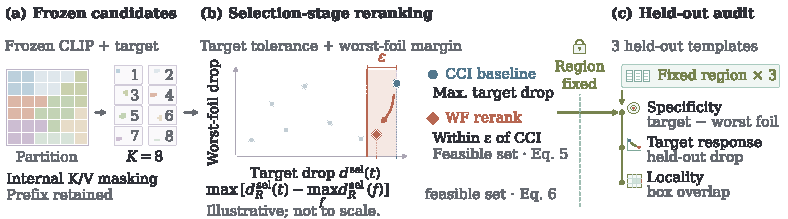
\includegraphics[width=\textwidth]{figures/figure1_method_clean.pdf}
\caption{Selection and held-out audit. A region is fixed using selection-stage
responses before three-template evaluation of specificity, target response,
and locality. The candidate-response diagram is illustrative, not measured data.}
\label{fig:method}
\end{figure*}

\section{Audit and Repair Opportunity}
For checkpoint $m$, $s_m(x,c)=\tau_m\langle z_m(x),e_m(c)\rangle$ is the
pre-softmax score with unit-norm embeddings and learned
$\tau_m=\exp(\ell_m)$. For a region $R$ and fixed internal intervention $\mathcal I$,
\begin{equation}
d_R(c)=s_m(x,c)-s_m(\mathcal I(x,R),c).
\label{eq:drop}
\end{equation}
Selection uses only ``a photo of a \{category\}'':
\begin{equation}
R_{\rm CCI}=\arg\max_{R\in\regions(x)}d_R^{\rm sel}(t).
\label{eq:cci}
\end{equation}

\paragraph{Held-out margins and screens.}
Evaluation uses ``a picture of the \{category\}'', ``an image containing a
\{category\}'', and ``the \{category\}''. For their unit-norm text embeddings,
let $n_c=\|H^{-1}\sum_h e_h(c)\|_2$, $\widetilde d_h(c)=d_h(c)/n_c$, and $H=3$.
The matched estimands are
\begin{equation}
\begin{aligned}
P_{\max}^{\rm pm}(R,t)&=H^{-1}\!\sum_h[\widetilde d_h(t)-\max_f\widetilde d_h(f)],\\
P_{\max}^{\rm agg}(R,t)&=H^{-1}\!\sum_h\widetilde d_h(t)-\max_f H^{-1}\!\sum_h\widetilde d_h(f).
\end{aligned}
\label{eq:estimands}
\end{equation}
The former allows a different hardest foil per template, so
$P_{\max}^{\rm pm}\le P_{\max}^{\rm agg}$. Below, $P=P_{\max}^{\rm agg}$ and
$\bar d_c=H^{-1}\sum_h\widetilde d_h(c)$. Aggregation equals using the
normalized mean text embedding; class-specific $n_c$ can change class rankings.

For the same CCI-top1 region, define
$A=\{\mathrm{bbox}\ge .5,\ \bar d_t-\mathrm{mean}_f\bar d_f>0\}$ and
$F=\{P<0\}$. The diagnostic screen and $.5$ threshold are study-defined,
not a standard of explanation validity. Because a positive mean-foil margin
does not require positive target drop, we also audit
$A^+=A\cap\{\bar d_t>0\}$. The primary repair population is
$B=A\cap F$, fixed before reranking. Negative $P$ is relative to the declared
foil ontology, not a judgment of semantic invalidity.

\paragraph{Target-constrained diagnostic probe.}
Define
\begin{equation}
M^{\rm sel}(R,t)=d_R^{\rm sel}(t)-\max_{f\in\foils_t}d_R^{\rm sel}(f),
\end{equation}
\begin{equation}
\regions_\epsilon=\{R:d_R^{\rm sel}(t)\ge d_{R_{\rm CCI}}^{\rm sel}(t)-\epsilon\},
\label{eq:feasible}
\end{equation}
and worst-foil (WF) reranking
\begin{equation}
R_{\rm WF}=\arg\max_{R\in\regions_\epsilon}M^{\rm sel}(R,t).
\label{eq:wf}
\end{equation}
The baseline is feasible, so any switch loses at most $\epsilon$ of
\emph{selection-stage} target drop; this gives no held-out guarantee.
Mean and Max-.1 instead maximize $d_t^{\rm sel}-\mathrm{mean}_f d_f^{\rm sel}$
and $d_t^{\rm sel}-.1\max_f d_f^{\rm sel}$ over the same set.
The fixed operating point is $.02$; a post-hoc $.01$--$.20$ sweep selects no
new optimum. Cosine-scale budgets $\epsilon/\tau_m$ are not calibrated
across checkpoints.

\paragraph{Exact diagnostic oracles.}
For a baseline-failure population $B$, the feasible repair count is
\begin{equation}
N_O(B,\epsilon)=\sum_{i\in B}\mathbf1\!\left\{
\max_{R\in\regions_\epsilon(i)}P_i(R)\ge0\right\}.
\label{eq:oracle}
\end{equation}
Replacing $\regions_\epsilon$ by all $K$ candidates gives the unrestricted
candidate oracle. A ``pass'' here means only $P_i(R)\ge0$, without a locality
or positive-target requirement. The disjoint classes are: no passing candidate
($C_0$); at least one passing candidate but \emph{none feasible} ($C_1$);
a feasible pass missed by WF ($C_2$); and WF sign repair ($r$).
Thus $|B|=C_0+C_1+C_2+r$ and $N_O=C_2+r$. We additionally count repairs
satisfying $J(R)=\{P_i(R)\ge0,\ A(R),\ \bar d_t(R)>0\}$; $A(R)$ applies
the same full-foil screen to the new region, without changing original $B$.
Oracles use held-out data only for diagnosis.

\paragraph{Fixed-population foil controls.}
For image $i$, let $\foils_i^{\rm abs}$ remove all annotated-present categories
from the non-target foils. Hold $R_{\rm CCI}$ and the full-foil screen $A$ fixed;
$F_i^{\rm abs}$ tests $\bar d_t-\max_{f\in\foils_i^{\rm abs}}\bar d_f<0$.
No region is reselected and no new mean screen is applied. A smaller foil set
cannot increase failure, so we also match its cardinality. For $N_i$ full
foils, $k_i=|\foils_i^{\rm abs}|$, and $m_i$ foils exceeding the target,
a uniform size-$k_i$ subset without replacement fails with probability
\begin{equation}
q_i=1-\frac{\binom{N_i-m_i}{k_i}}{\binom{N_i}{k_i}}.
\label{eq:matched}
\end{equation}
The numerator is zero when $k_i>N_i-m_i$. We compare
$\Delta_A=|A|^{-1}\sum_{i\in A}(\mathbf1\{F_i^{\rm abs}\}-q_i)$.
All restricted sets are nonempty. Annotation absence refers to retained
annotations, not verified semantic absence; COCO crowd categories remain excluded.

\section{Protocol and Reproducibility}
COCO val2014~\cite{lin2014coco} (27,708 images) and VOC2007
test~\cite{everingham2010voc} (1,943) pair with OpenAI CLIP B/16 and B/32,
yielding 59,302 image--model records. Targets are the largest instance's
category (COCO annotation area; VOC box area). Eligibility requires another
category and 2--80\% target area; COCO crowds are excluded.
Full foils are the other 79/19 classes.

OpenCLIP patch extraction uses \texttt{visual.\_pool} after the
transformer; projection uses \texttt{visual.proj}, then L2 normalization. K-means uses $K=8$, three
initializations, 50 iterations, and seed $1701+i$ for sample index $i$.
Masking blocks selected patch key/value columns in every block/head with
$-\infty$ before softmax, retaining the prefix. Ties use first argmax;
PyTorch 2.8.0 MPS features are cast to float32 before normalization.
BBox precision is the fraction of selected patch centers in target-class box unions,
mapped by $224/\min(W,H)$ and center-crop offsets; it measures neither pixel
precision nor target coverage~\cite{gomez2022metrics}.

Tables~\ref{tab:oracle}--\ref{tab:costs} reanalyze stored candidates using float32
selection arithmetic. Table~\ref{tab:screens} uses regenerated full-class responses:
all IDs, CCI labels, feasible sizes and full-foil states match; compared summaries
differ by less than $10^{-5}$. Each comparison fixes the regenerated region and
uses original scalars for $A,A^+$. Old masks are unavailable for byte comparison.

All intervals are 10,000-draw image bootstraps with NumPy \texttt{default\_rng}
and recorded deterministic seeds, using percentile 2.5/97.5 limits. Paired
quantities are differenced within image before resampling; intervals are
pointwise and unadjusted. Exact $q_i$ is primary; 100 seeded subset draws only
check it. Strategy/candidate arrays validate on all 59,302 records; a second
row-loop implementation independently checks oracle and tolerance counts.

\section{Results}
\begin{table}[!t]
\centering
\caption{Fixed original $A$: full-foil, annotation-absent, and exact cardinality-matched random failure rates (\%). $\Delta_A$ is absent minus random in percentage points, with paired 95\% CI.}
\label{tab:screens}
\small\setlength{\tabcolsep}{1.1pt}
\begin{tabular*}{\columnwidth}{@{\extracolsep{\fill}}lrrrr@{}}
\toprule
Setting & Full & Absent & Random & $\Delta_A$\\
\midrule
\tabinput{tables/restricted_rows.tex}
\bottomrule
\end{tabular*}
\end{table}

\paragraph{Failure persists after annotation exclusion.}
Screen sizes are 17,726, 17,847, 1,209, and 1,227 in table order.
Exclusion resolves only 213, 203, 16, and 17 full-foil failures;
96.63--98.24\% remain (failure counts in Table~\ref{tab:oracle}). The rate falls by 1.20/1.14/1.32/1.39 percentage
points. Table~\ref{tab:screens} separates this change from foil-count reduction:
COCO exclusion has a larger effect than random removal of the same number
of categories, whereas VOC $\Delta_A$ intervals include zero.
High failure is therefore not explained solely by explicitly annotated
co-occurring classes under this protocol.

\paragraph{Positive-target and scene-count checks.}
Requiring positive target drop leaves 16,855/17,330/1,186/1,215 images.
Full-foil failure in $A^+$ is 62.64/63.79/41.40/40.74\%; annotation-absent
failure remains 61.38/62.61/40.05/39.34\%. Matched-random comparisons retain
the COCO/VOC interval pattern. Even scenes with exactly two annotated
categories have COCO annotation-absent failure of 63.39/64.95\%.

\noindent\begin{minipage}{\columnwidth}
\centering
\captionof{table}{Exact local decomposition of \emph{screened failures} $B=A\cap F$
at $\epsilon=.02$. Counts in $C_0,C_1,C_2,r$ are mutually exclusive;
$C_2+r$ is the feasible-oracle count.}
\label{tab:oracle}
\small\setlength{\tabcolsep}{1.4pt}
\begin{tabular*}{\columnwidth}{@{\extracolsep{\fill}}lrrrrr@{}}
\toprule
Setting & $|B|$ & $C_0$ & $C_1$ & $C_2$ & $r$\\
\midrule
\tabinput{tables/oracle_rows.tex}
\bottomrule
\end{tabular*}
\end{minipage}\par\vspace{6pt}

\paragraph{Candidate and budget bottlenecks differ by dataset.}
No region among the eight candidates passes for 93.75/92.16\% of COCO
screened failures, versus 72.60/68.71\% on VOC (Table~\ref{tab:oracle}).
Removing the budget would therefore permit sign repair in only 6.25/7.84\%
of COCO $B$, versus 27.40/31.29\% on VOC. These limits concern the stored
candidates, not every possible image region. The $.02$ budget then excludes
96.43--98.10\% of those unrestricted opportunities: for COCO B/16, 695 of
713 are excluded, leaving 18. Across settings, feasible-oracle counts are
18/31/5/3 (0.16/0.27/0.98/0.59\% of $B$), and WF finds 18/30/5/2.
Scarce passing candidates and budget exclusion dominate; few feasible
repairs are missed, although VOC event counts are small.

\newpage

\noindent\begin{minipage}{\columnwidth}
\centering
\captionof{table}{Local COCO B/16 tolerance sweep. Multi is the all-image percentage
with $|\regions_\epsilon|>1$; $O_B,r_B$ are oracle/actual repair percentages
\emph{of fixed $B$}. Target and bbox columns show \emph{global impacts}: all-image WF$-$CCI
means, not costs conditional on repair. Bbox is in percentage points.}
\label{tab:frontier}
\small\setlength{\tabcolsep}{1pt}
\begin{tabular*}{\columnwidth}{@{\extracolsep{\fill}}rrrrrr@{}}
\toprule
$\epsilon$ & Multi & $O_B$ & $r_B$ & $\Delta d_t$ & $100\Delta$bbox\\
\midrule
\tabinput{tables/frontier_rows.tex}
\bottomrule
\end{tabular*}
\end{minipage}\par\vspace{6pt}

\paragraph{More opportunity requires a looser budget.}
In Table~\ref{tab:frontier}, increasing $\epsilon$ from $.02$ to $.20$
raises the multi-candidate fraction from 4.71\% to 35.78\% and screened-failure
oracle repair from 0.16\% to 1.57\%. Mean selection-target loss rises from
$.000245$ to $.023805$. At $.20$, held-out raw target change is
$-.01397$ $[-.01520,-.01275]$, and bbox change is $-1.63$ points
$[-1.88,-1.37]$. The four-setting sweep is released; at $.20$,
$O_B$ is 2.05/6.65/7.13\% for COCO B/32 and VOC B/16/B/32.
The tight-budget bottleneck is thus not invariant to tolerance.

\noindent\begin{minipage}{\columnwidth}
\centering

\includegraphics[width=\columnwidth]{figures/figure2_identification_final.pdf}
\captionof{figure}{Frozen-archive normalized aggregate margin gains at $\epsilon=.02$;
bars are paired 95\% CIs. Disjoint-category and annotation-absent evaluation
retain gains for a fixed selection/evaluation protocol.}
\label{fig:ident}
\end{minipage}\par\vspace{6pt}

\paragraph{Global impact is not the cost of repair.}
Table~\ref{tab:frontier} averages costs over all images, including unchanged
regions. Within $B$, the 254/270/16/7 switches at $.02$ instead have mean bbox
changes of $-28.80/-24.92/-39.60/-35.52$ points. Table~\ref{tab:costs}
is narrower still: it conditions on actual sign repairs in $B$.
The released five-budget analysis separates both subsets. Their conditional
costs must not be interpreted as all-image effects or causal treatment effects.

\newpage

\noindent\begin{minipage}{\columnwidth}
\centering
\captionof{table}{Local paired margin gains, WF minus the alternative, with 95\% CIs;
values multiplied by $10^3$. $D$ counts WF/Max-.1 selection disagreements.}
\label{tab:baselines}
\small\setlength{\tabcolsep}{1pt}
\begin{tabular*}{\columnwidth}{@{\extracolsep{\fill}}lrrr@{}}
\toprule
Setting & WF$-$Mean & WF$-$Max-.1 & $D$\\
\midrule
\tabinput{tables/comparison_rows.tex}
\bottomrule
\end{tabular*}
\end{minipage}\par\vspace{6pt}

\paragraph{Small baseline gains arise from few disagreements.}
WF and Max-.1 differ on only 84/89/5/5 images
(Table~\ref{tab:baselines}). Their agreement is over 99.6\% overall but
93.56/92.70/94.62/94.57\% within multi-candidate sets.
On the 84 COCO B/16 disagreements, WF gains $.0807$ margin
$[.0443,.1171]$, while raw target drop changes by $-.0326$
$[-.0628,-.0033]$. The whole-sample gain is $.000245$.
The VOC disagreement subsets contain only five images each.

\noindent\begin{minipage}{\columnwidth}
\centering
\captionof{table}{Actual sign repairs \emph{within original $B$}, $\epsilon=.02$.
$r$ counts repairs; $j$ counts those also satisfying $J$.
WF$-$CCI means and repair-subset 95\% CIs; raw target drop, bbox in percentage points.}
\label{tab:costs}
\small\setlength{\tabcolsep}{1.1pt}
\begin{tabular*}{\columnwidth}{@{\extracolsep{\fill}}lrrrr@{}}
\toprule
Setting & $r$ & $j$ & $\Delta d_t$ & $100\Delta$bbox\\
\midrule
\tabinput{tables/endpoint_cost_rows.tex}
\bottomrule
\end{tabular*}
\end{minipage}\par\vspace{6pt}

\paragraph{Sign repair need not retain the other endpoints.}
Only 12/25/3/1 of the 18/30/5/2 repairs in $B$ also retain the original
screen and positive target contribution (Table~\ref{tab:costs}). The joint
feasible-oracle counts are 12/26/3/2. Small VOC repair subsets make their
cost intervals descriptive, not evidence of stable population effects.
Across \emph{all baseline failures}, WF sign-repairs 42/48/11/6 cases;
0/4/0/0 opposite-sign regressions leave net reductions of 42/44/11/6.
Across all 663/614/50/38 switches, 611/532/46/35 improve margin, with
B/16 bbox changes of $-4.95/-13.20$ points on COCO/VOC.
These are different populations from $B$ repairs. Raw-target intervals
containing zero do not establish equivalence.

\newpage

\noindent\begin{minipage}{\columnwidth}
\centering
\setlength{\fboxsep}{6pt}
\fbox{\begin{minipage}{\dimexpr\columnwidth-2\fboxsep-2\fboxrule\relax}
\centering
\textbf{Local screen-passing failure and repair}\\[3pt]
COCO B/16, image 254807: \textbf{person}\\
CCI hardest foil: \emph{tie} (annotation-absent)\\[5pt]
\small
\begin{tabular*}{\linewidth}{@{\extracolsep{\fill}}lrr@{}}
\toprule
Endpoint & CCI-top1 & WF\\
\midrule
Worst-foil margin $P$ & $-.6545$ & $+.2689$\\
Mean-foil margin & $+.0216$ & $+.9090$\\
Raw target drop & $+.3462$ & $+.3633$\\
BBox precision & $.7143$ & $.6111$\\
\bottomrule
\end{tabular*}\par\vspace{5pt}
\normalsize
$A^+\cap F$ before $\longrightarrow$ $J$ after\\
Sign repaired; locality remains above $.5$ but falls.
\end{minipage}}
\captionof{figure}{A local $A^+\cap F$ case, selected by median baseline margin
among 17 COCO B/16 $A^+\cap F$ sign repairs. Margins use each region's own
full-foil maximum; the named foil is for CCI. This response audit shows absolute
endpoints, not reconstructed masks or event frequency.}
\label{fig:cases}
\end{minipage}\par\vspace{6pt}

\section{Scope and Conclusion}
Removing annotated co-occurring classes leaves high failure rates and has a
measurable effect beyond cardinality on COCO. This does not establish complete
annotation, semantic error, or a causal account of the response vector.
The results concern two datasets, two checkpoints, eight candidates and one
intervention. Raw worst-foil/normalizer sensitivity and region-size/segmentation
controls remain untested.

The \href{https://github.com/jovial-liu/conway/tree/1817e1666161fa902869affe61b55f7c98c45668/experiments}{original local inputs}
are pinned to \texttt{1817e166}; the
\href{https://github.com/jovial-liu/conway/tree/6a52e8f3d39f343d8483390882dcb5e57003d904/experiments/reviewer_controls_2026-09-13}{restricted-foil controls}
to \texttt{6a52e8f3}. Independent local verification reads full responses;
our portable check redoes all 40 reported foil intervals from released per-image
diagnostics. Full-class tensors remain local with published hashes, permitting
summary reanalysis but not independent recovery of arbitrary class subsets from
the public diagnostics alone. Frozen tensors and old candidate masks are
incomplete; numerical agreement is not backend or mask equivalence.
The \texttt{ccf0-round4-20260914} package adds losslessly stored candidate
responses for all eight regions, an independent endpoint checker, and
subset-cost tables. It maps all five main tables to fixed inputs and code;
selected-region full-class vectors still require the local response archives.

The main findings are persistent screened violations after annotation exclusion
and dataset-dependent repair bottlenecks. COCO has fewer unrestricted passing
candidates than VOC; the tight target budget excludes most remaining
opportunities in both. WF misses few feasible sign repairs, but some repairs
lose locality or positive target evidence. A looser budget increases opportunities
and global costs. Keeping populations and endpoints separate is therefore
central to interpreting CCI-top1 audits, rather than judging an entire heatmap.

\clearpage
\balance
\input{references.tex}
\end{document}
